
\documentclass[aspectratio=1610, 13pt]{beamer}
\usepackage{ctex}
\usepackage{CJKutf8}

\setCJKmainfont[ItalicFont=Noto Sans CJK SC Bold, BoldFont=Noto Serif CJK SC Black]{Noto Serif CJK SC}

\usepackage{xcolor}
\usepackage{multicol}
\usepackage{mathtools,array}
\usepackage[T1]{fontenc}
\usepackage{zi4}
\usepackage[font={scriptsize,bf}]{caption}
% \usepackage{subcaption}
\usepackage{graphics}
\usepackage{tikz}
\usepackage{fontawesome5}
\usepackage{mathpartir}

\newcommand{\naturals}{\mathbb{N}}
\newcommand{\reals}{\mathbb{R}}

\newcommand{\Dist}[1]{\mathcal{D}(#1)}
\newcommand{\expectation}{\mathbb{E}}

\newcommand{\states}{S}
\newcommand{\actions}{A}
\newcommand{\observables}{O}
\newcommand{\trans}{T}
\newcommand{\obs}{Z}
\newcommand{\reward}{R}
\newcommand{\discount}{\gamma}

\newcommand{\beliefs}{\mathcal{B}}
\newcommand{\beliefUpdate}{\tau}

\newcommand{\policy}{\pi}

\newcommand{\diff}[1]{\mathop{}\!\mathrm{d}#1}
\renewcommand{\figurename}{Figure}
\renewcommand{\refname}{Reference}

\AtBeginDocument{
  \catcode`_=12
  \begingroup\lccode`~=`_
  \lowercase{\endgroup\let~}\sb
  \mathcode`_="8000
}

% \usetheme{Madrid}
% % \usetheme{default}
% \setbeamertemplate{caption}[numbered]
% \setbeamerfont{title}{size=\large}
\mode<presentation>
{
  \usetheme{Darmstadt}      % or try Darmstadt, Madrid, Warsaw, ...
  \usecolortheme{default} % or try albatross, beaver, crane, ...
  \usefonttheme[onlymath]{serif}  % or try serif, structurebold, ...
  \setbeamertemplate{navigation symbols}{}
  \setbeamertemplate{caption}[numbered]
  \setbeamertemplate{footline}[frame number] 
} 

\usepackage{listings}
\lstdefinestyle{heaplang}{
    language=C,
    basicstyle=\footnotesize\ttfamily,
    keywordstyle=\color{blue},
    commentstyle=\color{red},
    escapeinside={<@}{@>},
    morekeywords={new_chan, fork, recv, send, swap, ref}
}
\lstdefinestyle{clang}{
    language=C,
    basicstyle=\footnotesize\ttfamily,
    keywordstyle=\color{blue},
    commentstyle=\color{red},
    escapeinside={<@}{@>},
}
\lstset{style=heaplang}

\usepackage{natbib}

\newcommand{\buchi}{B\"uchi }

\definecolor{goldenpoppy}{rgb}{0.99, 0.76, 0.0}
\definecolor{goldenyellow}{rgb}{1.0, 0.87, 0.0}
\definecolor{green2}{rgb}{0.1,0.7,0.3} 
\newcommand{\gcheck}{{\color{green2}\faCheckCircle[regular] }}
\newcommand{\rcross}{{\color{red} \faTimesCircle[regular]} }
\newcommand{\rflag}{{\color{red} \faFlag}}
% \usepackage{algorithm,amsmath}
% \usepackage[noend]{algpseudocode}

\newcommand{\zlstinline}{\let\par\endgraf\lstinline}
\newcommand{\comments}[1]{{\color{red}#1}}
\title{Group Meeting}
\date{\today}
\author{Members: Yong Li, Depeng Liu, Weizhi Feng, Xie Li, Shizhen Yu, Yutian Zhu, Zongxin Liu}
\begin{document}
\maketitle

\begin{frame}\frametitle{差分隐私——刘德鹏}
这周:
\begin{itemize}
  \item 连续机制建模:阅读强化学习5/6/7章节,讨论了转移到差分隐私中建模及遇到的难点:连续空间event转化为action的处理,reward分配等;
  \item Pufferfish 文章:工具比较需更新,验证工具(CheckDP,20 'CCS)不能直接适用于离散噪声场景,适用于黑盒场景的基于机器学习工具(DP-Sniper,21 'SP)应该会适用,在读文章(DP-Sniper: Black-Box Discovery of Differential Privacy Violations using Classifiers,21 'SP),其根据DP机制的输入、输出训练分类器,拟合给定输出在输入下的后验分布,来寻找最可能违反DP的反例。
  \item 参数选取:调研了 最早的一篇How much is enough? choosing $\epsilon$ for differential privacy(11’ ISC)文章,相同大小的$\epsilon$对于不同机制、数据域、查询的影响不同,表现为推断真实数据的分布的影响,是一个相对意义的参数,其选取比设计隐私机制甚至更有挑战。存在局限性为没有正确认清背景知识对差分隐私的保护削弱影响,只能在小案例上分析等。
\end{itemize}

计划:
\begin{itemize}
  \item 强化学习教材阅读,考虑最简单连续机制的建模;
  \item 精读21 'SP的文章,调研工具使用;
  \item 参数选取更多文章调研。
\end{itemize}
\end{frame}
\begin{frame}\frametitle{内存安全——李勰、刘宗鑫}
上周计划(进行中):
\begin{itemize}
\item 根据SV-COMP加入库函数语义的支持。
\item 代码的重构。
\item 继续跑例子进行测试和Debug。
\end{itemize}

SV-COMP:
\begin{center}
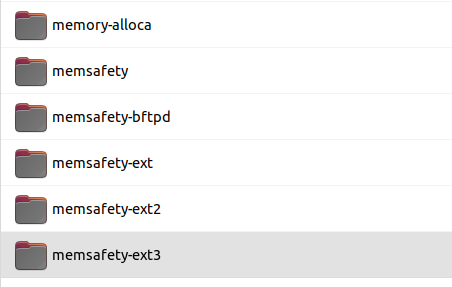
\includegraphics[scale=0.4]{sv1.png}
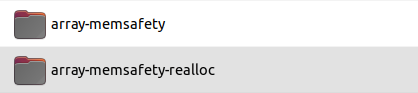
\includegraphics[scale=0.4]{sv2.png}
\end{center}
选取用例:memsafety文件夹共38个例子



\end{frame}

\begin{frame}\frametitle{内存安全——李勰、刘宗鑫}
在38个例子中:
\begin{itemize}
\item Successfully verified: 2 $\rightarrow$ 10
\item Unmatched result: 2 $\rightarrow$ 3
\item Exceptions raised: 34 $\rightarrow$ 25
\end{itemize}

其中Unmatched result中,目前有1个误报,2个漏报。


TODOs:
\begin{enumerate}
\item 寻找误报漏报原因,特别是误报,可能是因为语义的bug.
\item 继续添加对SV-COMP的支持和Debug.
\item \textbf{优化问题:}部分例子运行时间过长,50s左右
\item 给出更具体的内存安全问题的划分,目前只是给出UNSAFE结果。
\end{enumerate}
\end{frame}
\begin{frame}{冯维直}
    \begin{itemize}
        \item 期刊文章:
        \begin{itemize}
            \item [-] 上周计划是将SDBA取补算法正确性证明写完,然后增加一个determinization (确定化,给定SDBA, 构建一个DRA) 的章节,目前完成进度:SDBA取补算法正确性写完了;determinization构造写完了.
        \end{itemize}
        \item 阅读
        \begin{itemize}
            \item [-] 看之前CAV的一篇文章decoupled search做composed \buchi automata 的liveness verification,还没看完,计划下下周三组会的时候报告.
        \end{itemize}
        \item 计划
        \begin{itemize}
            \item [-] 期刊文章根据实验情况写实验部分.
            \item [-] 读CAV文章.
            \item [-] 读程序分析教材3.1 3.2节,根据硬件验证小组要求读相关内容:chisel验证;或者handbook of modelchecking相关章节.
        \end{itemize}
\end{itemize}    
\end{frame}


\begin{frame}
  \frametitle{朱雨田}
  \begin{itemize}
      \item 调研了VeriSolid的建模模块,即FSolidM。
      \begin{itemize}
        \item 函数体的语句不能自动生成,需要手动输入。
        \item SolidM对于constructor和fallback不能很好地支持。
        \item 不支持多合约交互建模。
      \end{itemize}
      \item VerX: Safety Verification of Smart Contracts(读了一半左右)
      \item 下周计划:
      \begin{itemize}
        \item 继续调研VeriSolid,考察FSolidM的建模功能和阅读对应源码。
        \item 准备讨论班。
        \item 有时间就熟悉一下smack项目。
      \end{itemize}
  \end{itemize}
\end{frame}

\begin{frame}{
\includegraphics[scale=0.23]{ysz6.png}}


进展:
    \begin{itemize}
        \item 上周读了《 Learning Deterministic Automata on InfiniteWords》,跟李老师周末大概讲了讲主要的思路,文章中的一些证明细节也基本上弄清楚了。 
        \item 这周在读《 Boolean Satisfiability Solvers and Their Applications in Model Checking》,现在大概通读完一遍,再整理整理,明天做一下汇报。
\end{itemize}    
\end{frame}



\end{document}